
\begin{figure}[htbp]
\centering
\begin{tikzpicture}[font=\small, x=0.86cm, y=0.68cm]
  \node[anchor=east] at (0,3) {PU$_1$};
  \node[anchor=east] at (0,2) {PU$_2$};
  \node[anchor=east] at (0,1) {PU$_3$};
  \draw[->] (0,0.35) -- (10.3,0.35) node[right] {idő};
  \foreach \x in {1,...,10} {\draw[black!20] (\x,0.25) -- (\x,3.45);}
  \draw[fill=lightaccent, draw=accent] (0.2,2.75) rectangle (2.4,3.25) node[pos=.5] {$A$};
  \draw[fill=warnbg, draw=orange!70!black] (2.4,2.75) rectangle (4.3,3.25) node[pos=.5] {$B$};
  \draw[fill=black!8, draw=black!50] (4.3,2.75) rectangle (5.4,3.25) node[pos=.5] {$C$};
  \draw[fill=lightaccent, draw=accent] (1.0,1.75) rectangle (3.8,2.25) node[pos=.5] {$D$};
  \draw[fill=warnbg, draw=orange!70!black] (3.8,1.75) rectangle (6.2,2.25) node[pos=.5] {$E$};
  \draw[fill=lightaccent, draw=accent] (5.0,0.75) rectangle (8.0,1.25) node[pos=.5] {$F$};
  \node[align=center] at (5,-0.55) {Gantt-diagram: megmutatja, hogy melyik számítási egység mikor dolgozik.};
\end{tikzpicture}
\hfill
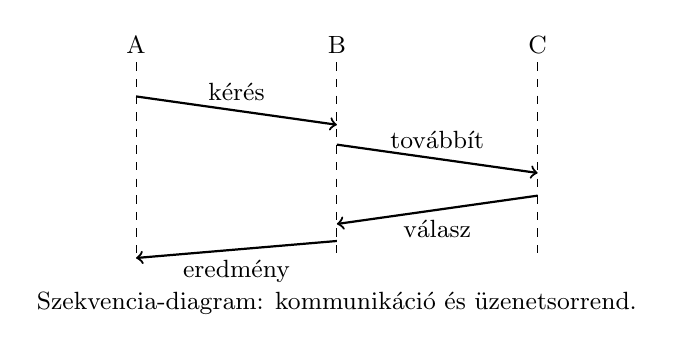
\begin{tikzpicture}[font=\small, x=0.85cm, y=0.72cm]
  \node at (0,4) {A};
  \node at (3,4) {B};
  \node at (6,4) {C};
  \draw[dashed] (0,3.7) -- (0,0.3);
  \draw[dashed] (3,3.7) -- (3,0.3);
  \draw[dashed] (6,3.7) -- (6,0.3);
  \draw[->, thick] (0,3.1) -- node[above] {kérés} (3,2.6);
  \draw[->, thick] (3,2.25) -- node[above] {továbbít} (6,1.75);
  \draw[->, thick] (6,1.35) -- node[below] {válasz} (3,0.85);
  \draw[->, thick] (3,0.55) -- node[below] {eredmény} (0,0.25);
  \node[align=center] at (3,-0.55) {Szekvencia-diagram: kommunikáció\ és üzenetsorrend.};
\end{tikzpicture}
\caption{Két gyakori ábrázolás: Gantt-diagram és szekvencia-diagram}
\label{fig:zv07_gantt_szekvencia}
\end{figure}
